%%%%%%%%%%%%%%%%%%%%%%%%%%%%%%%%%%%%%%%%%%%%%%%%%%%%%%%%%%
\begin{frame}
  \begin{center}
    {\Large Data Visualization}
  \end{center}
\end{frame}


%%%%%%%%%%%%%%%%%%%%%%%%%%%%%%%%%%%%%%%%%%%%%%%%%%%%%%%%%%
\begin{frame}[fragile]\frametitle{Visualizations}	
\begin{itemize}
\item The display of information in a graphic or tabular format.
\item Many visualization formats exist (contour plots, graphs, heat maps) to display high-dimensional information.
\item Since this isn't a visualization course, we'll mainly use ``traditional'' two-dimensional graphic types.
\item How can we transform a dataset with many attributes into two dimensions?
\begin{itemize}
\item Selection: Typically by selecting two dimensions at a time
\item Can also only ``select'' subset of records to display
\item Other techniques also exist
\end{itemize}
\end{itemize}
\end{frame}

%%%%%%%%%%%%%%%%%%%%%%%%%%%%%%%%%%%%%%%%%%%%%%%%%%%%%%%%%%
\begin{frame}[fragile]\frametitle{Visualizations}	
\begin{itemize}
\item Data visualization is not just making fancy graphics for reports; it is used extensively in day-to-day work for all phases of a project.
\item We do preliminary checks and analysis using graphics and tables to summarize the data and leave out the less important details.
\item when we analyze the performance of a model or report results, we also often use charts and images. 
\item Sometimes, for interpreting a complex model, we need to project high-dimensional spaces onto more visually intelligible 2D or 3D figures.
\end{itemize}
\end{frame}

%%%%%%%%%%%%%%%%%%%%%%%%%%%%%%%%%%%%%%%%%%%%%%%%%%%%%%%%%%
\begin{frame}
  \begin{center}
    {\Large Sample:Iris Data Set }
  \end{center}
\end{frame}

%%%%%%%%%%%%%%%%%%%%%%%%%%%%%%%%%%%%%%%%%%%%%%%%%%%%%%%%%%
\begin{frame}[fragile]\frametitle{Dataset Information}	
\begin{itemize}
\item Freely available from UCI (University of California at Irvine) Machine Learning Lab
\item Relatively very small
\item 150 records of Iris flowers (50 for each species)
\item Attributes:
\begin{itemize}
\item Sepal length (centimeters)
\item Sepal width (centimeters)
\item Petal length (centimeters)
\item Petal width (centimeters)
\item Class (species of Iris) {Setosa, Versicolour, Virginica}
\end{itemize}
\end{itemize}
\end{frame}


%%%%%%%%%%%%%%%%%%%%%%%%%%%%%%%%%%%%%%%%%%%%%%%%%%%%%%%%%%
\begin{frame}[fragile]\frametitle{Visualization: Histogram}	
\begin{itemize}
\item For showing the distribution of values
\item Divide values into bins; show number of objects that fall into each bin
\item Shape of histogram depends on number of bins
\item For categorical attributes, each category is a bin
\end{itemize}
\begin{center}
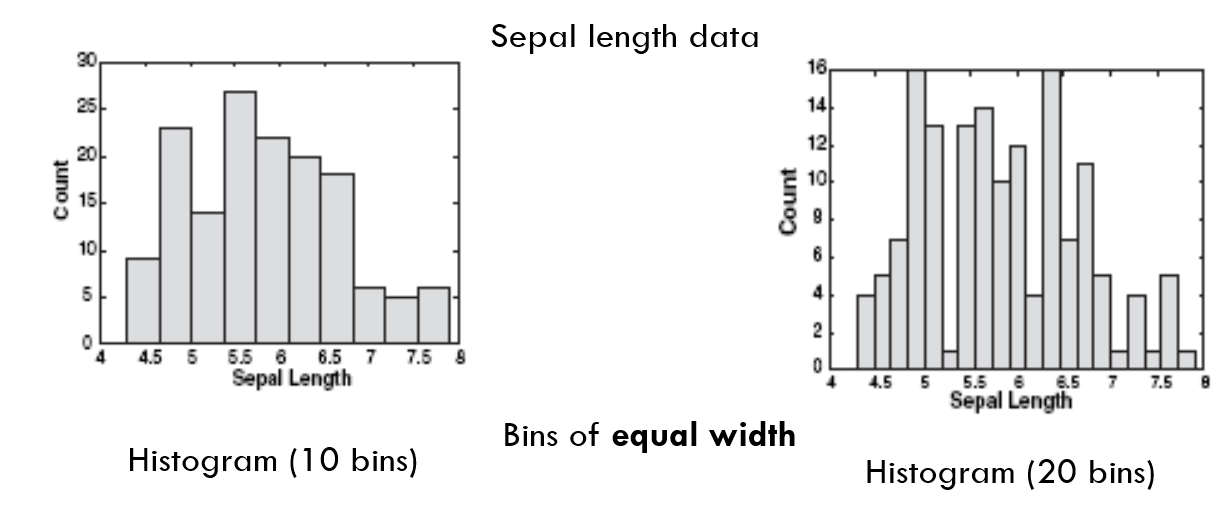
\includegraphics[width=0.8\linewidth,keepaspectratio]{histogram}
\end{center}
\end{frame}


%%%%%%%%%%%%%%%%%%%%%%%%%%%%%%%%%%%%%%%%%%%%%%%%%%%
\begin{frame}[fragile] \frametitle{Visualization: Box Plot}

\adjustbox{valign=t}{
\begin{minipage}{0.45\linewidth}
\begin{center}
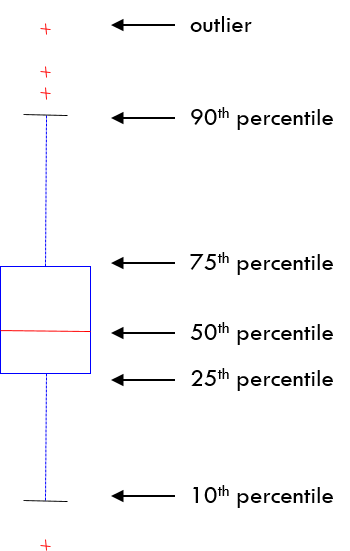
\includegraphics[width=\linewidth,keepaspectratio]{boxplot}
\end{center}
\end{minipage}
}
\hfill
\adjustbox{valign=t}{
\begin{minipage}{0.45\linewidth}
\begin{itemize}
\item Box plots show the distribution of the values for a single numerical attribute.
\item Whiskers: top and bottom lines of the box plot
\item Whiskers can represent several possible alternate values
\item Best to describe the convention used in a legend along the chart
\end{itemize}
\end{minipage}
}
\end{frame}

%%%%%%%%%%%%%%%%%%%%%%%%%%%%%%%%%%%%%%%%%%%%%%%%%%%
\begin{frame}[fragile] \frametitle{Iris: Box Plot}
Box plots are relatively compact; many of them can be shown on the same plot.

\begin{center}
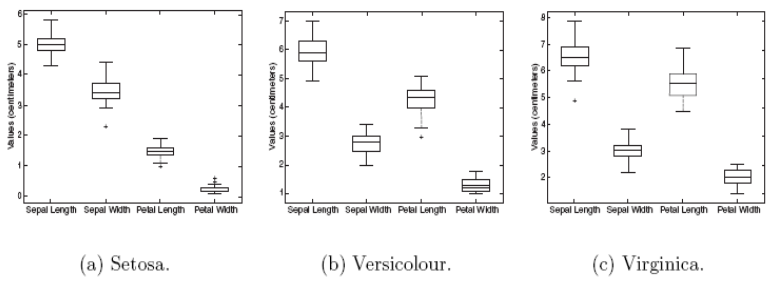
\includegraphics[width=0.8\linewidth,keepaspectratio]{irisbox}
\end{center}

\end{frame}

%%%%%%%%%%%%%%%%%%%%%%%%%%%%%%%%%%%%%%%%%%%%%%%%%%%%%%%%%%
\begin{frame}[fragile]\frametitle{Visualization: Scatter Plot}	
\begin{itemize}
\item Data objects are plotted as a point in a 2d-plane: one attribute on x-axis, the other on y-axis
\item Assumed that both attributes are discrete or continuous
\item Scatter plot matrix: organized way to examine a number of scatter plots simultaneously
\item Scatter plots for multiple pairs of attributes
\end{itemize}
\end{frame}

%%%%%%%%%%%%%%%%%%%%%%%%%%%%%%%%%%%%%%%%%%%%%%%%%%%
\begin{frame}[fragile] \frametitle{Iris: Scatter}
When class labels are available, a scatter plot matrix can visualize how much two attributes separate the classes.


\begin{center}
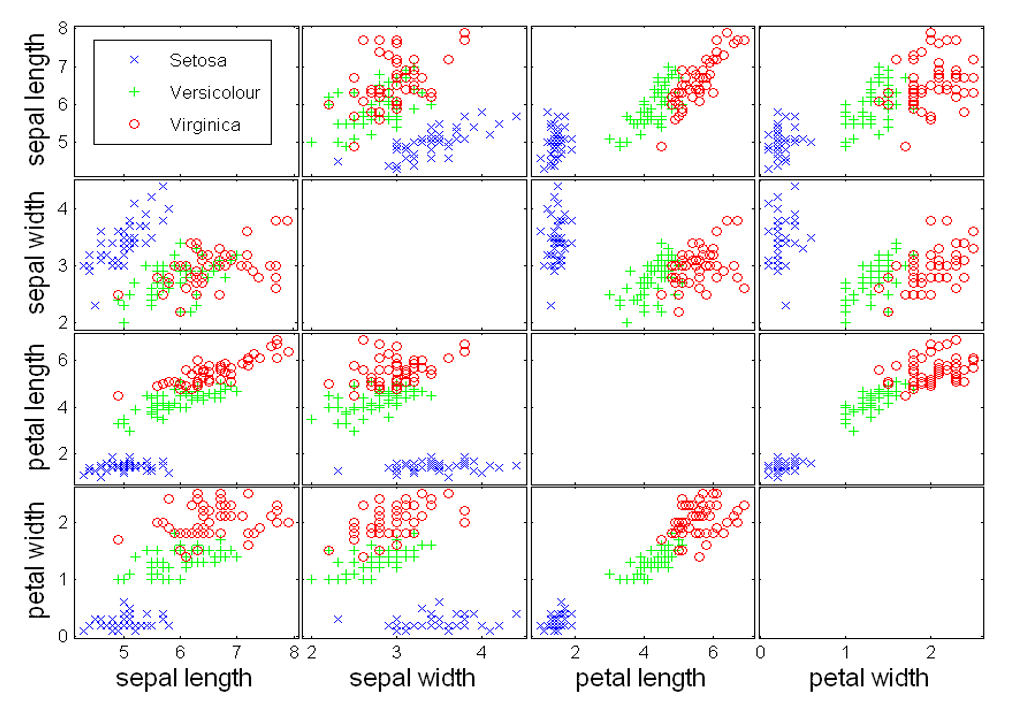
\includegraphics[width=0.8\linewidth,keepaspectratio]{irisscatter}
\end{center}

\end{frame}
